\section[q5]{Question 5}
\textit{Assessing whether air pollution levels are above the WHO recommended guidelines
is imperative for determining the association between health and air pollution at a
population level. Is there an association between who\_region and the air pollution
exposure categories created in Assignment 1 [pick a single year in which to investig-
ate the association]?}

\subsection{Question 5.a}
\textit{Plot a single bar graph showing the relationship between these two variables.}\\

In 2020, only four regions submitted $PM_{2.5}$ concentration data to the WHO.  Figure \ref{fig:q5_bar_pm25_region} shows the $PM_{2.5}$ concentration categories by WHO region for 2020. The regions are colour-coded according to the air pollution exposure categories created in Assignment 1.

\begin{figure}[H]
    \centering
    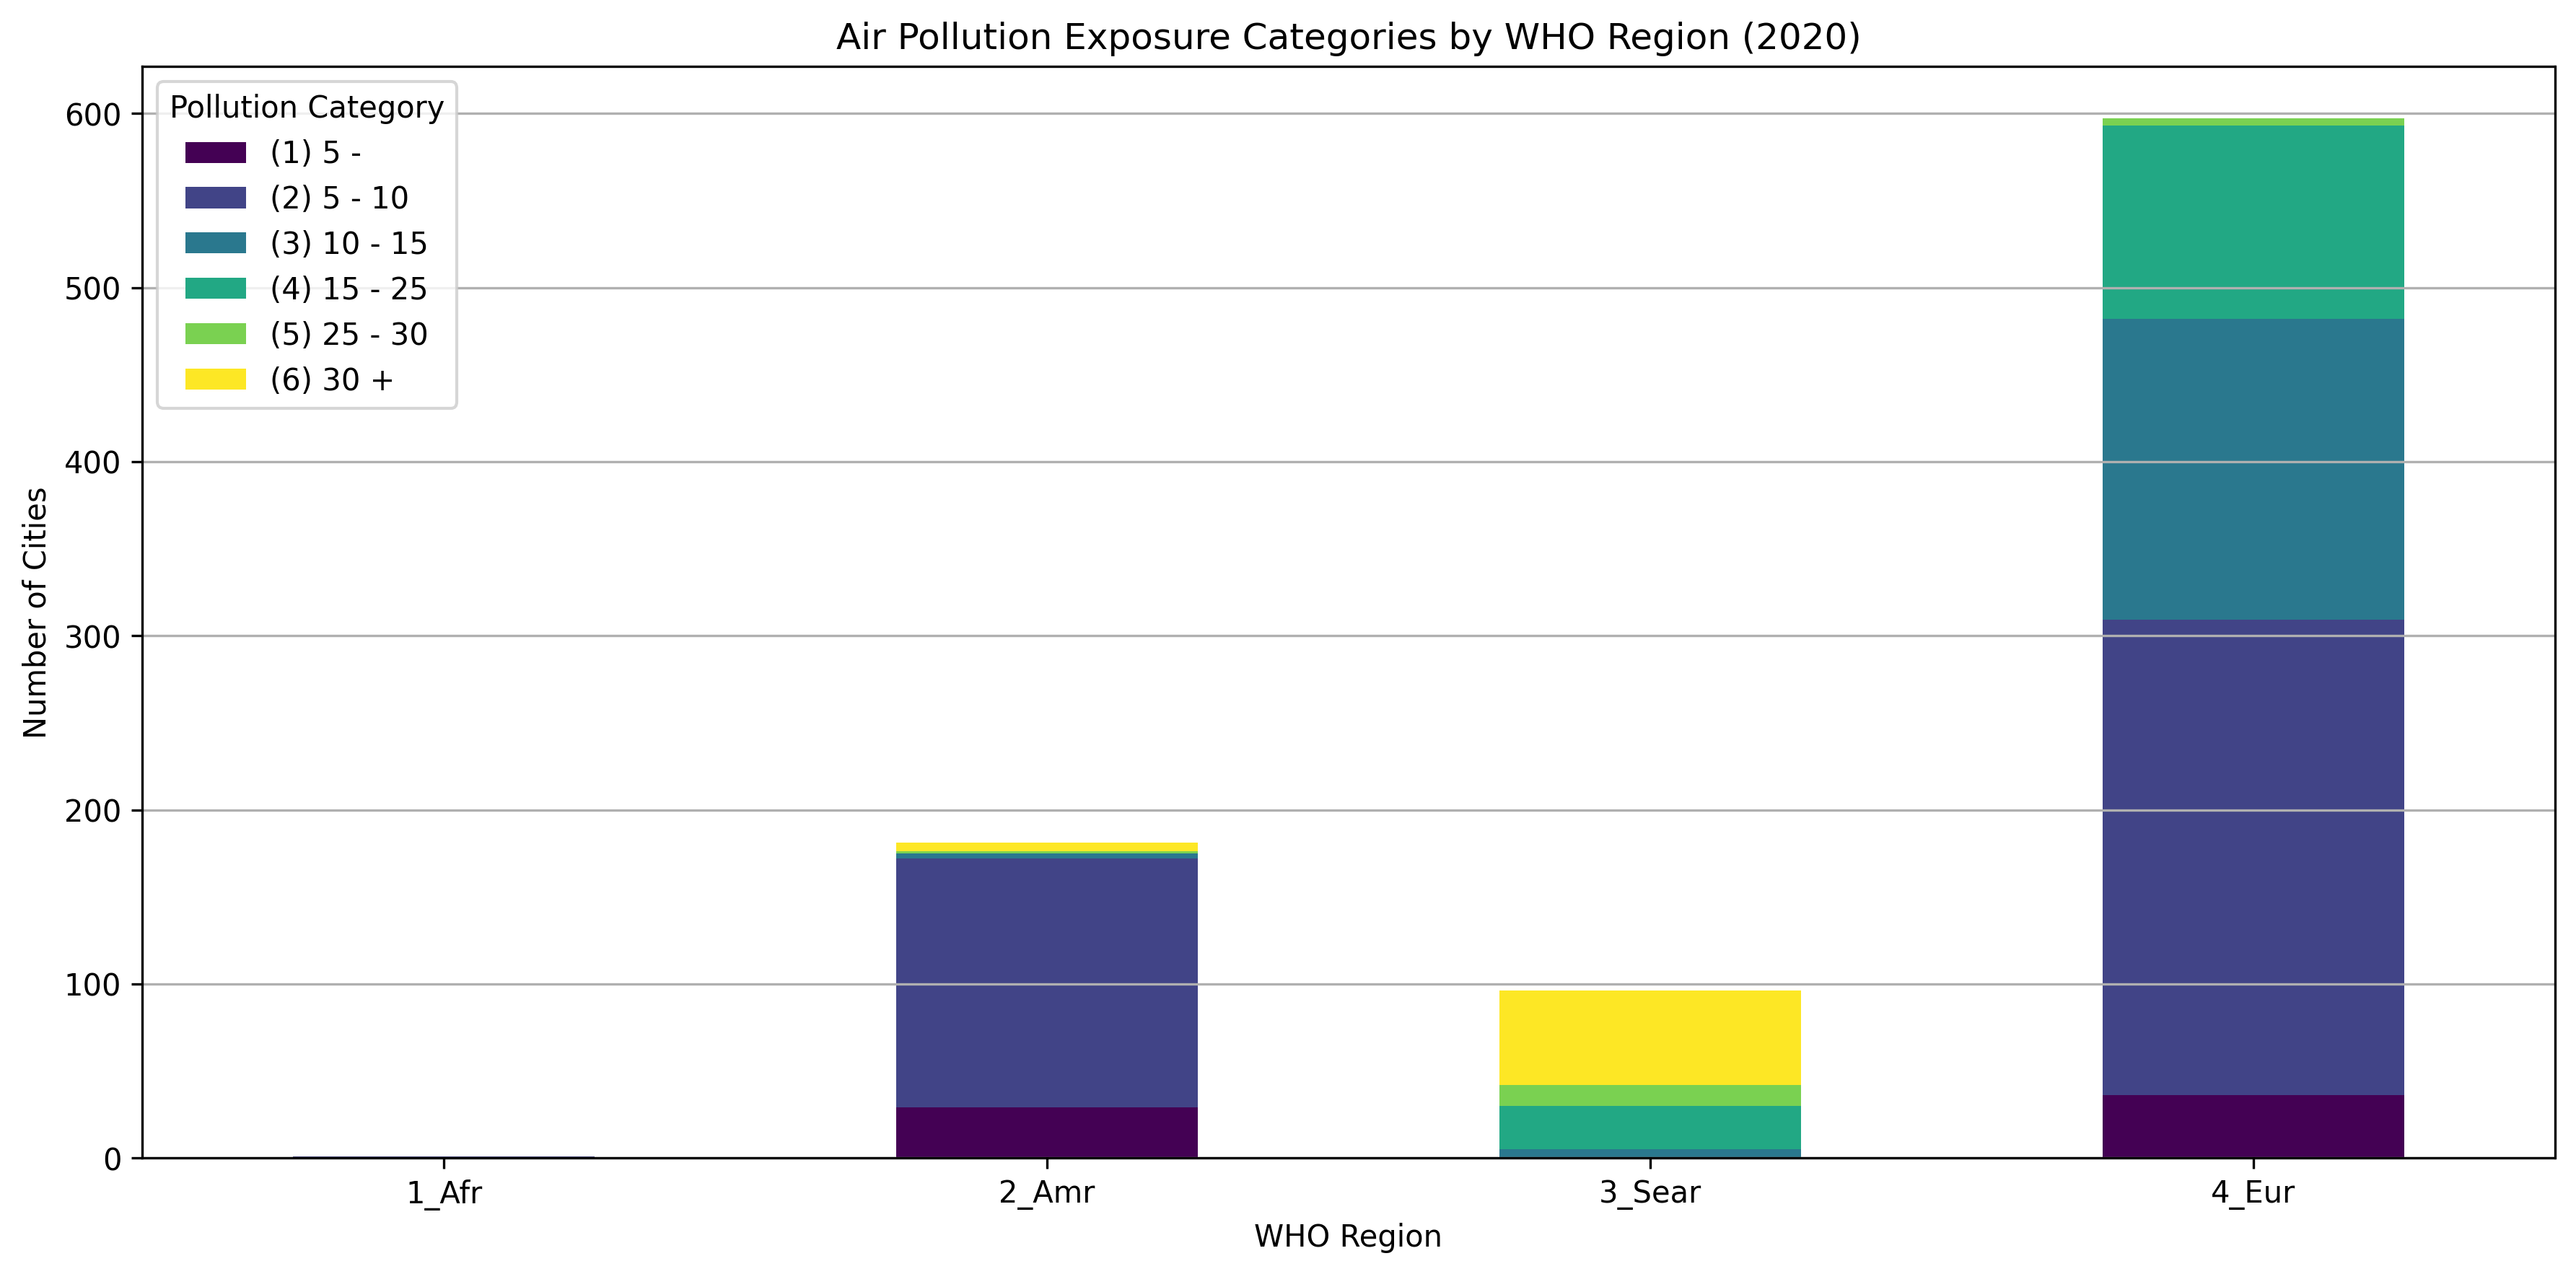
\includegraphics[width=0.8\textwidth]{img/q5_bar_pm25_region.png}
    \caption{$PM_{2.5}$ concentration by WHO region - 2020.}
    \label{fig:q5_bar_pm25_region}
\end{figure}

\subsection{Question 5.b}
\textit{What is the prevalence of the highest air pollution exposure category you created?}
\begin{itemize}
    \item \textit{In your overall sample?}
    \item \textit{In the 4\_Eur who\_region?}
    \item \textit{In the 1\_Afr who\_region?}
\end{itemize}

\textit{Report your answers in written sentences (not just reporting number). Hint: refer to your descriptive table or make a new 2x2 table to help you answer this.}


% \begin{tabular}{lrrrrrrr}
%     \toprule
%     pm25\_cats & (1) 5 - & (2) 5 - 10 & (3) 10 - 15 & (4) 15 - 25 & (5) 25 - 30 & (6) 30 + & Total \\
%     who\_region &  &  &  &  &  &  &  \\
%     \midrule
%     1\_Afr & 0 & 1 & 0 & 0 & 0 & 0 & 1 \\
%     2\_Amr & 29 & 143 & 3 & 0 & 1 & 5 & 181 \\
%     3\_Sear & 0 & 0 & 5 & 25 & 12 & 54 & 96 \\
%     4\_Eur & 36 & 273 & 173 & 111 & 4 & 0 & 597 \\
%     Total & 130 & 834 & 362 & 272 & 34 & 118 & 1750 \\
%     \bottomrule
%     \caption{Descriptive statistics for WHO regions overall and by year}
% \end{tabular}\\

\begin{table}[ht]
    \centering
    \begin{tabular}{lrrrrrrr}
        \toprule
        pm25\_cats & (1) 5 - & (2) 5 - 10 & (3) 10 - 15 & (4) 15 - 25 & (5) 25 - 30 & (6) 30 + & Total \\
        who\_region &  &  &  &  &  &  &  \\
        \midrule
        1\_Afr & 0 & 1 & 0 & 0 & 0 & 0 & 1 \\
        2\_Amr & 29 & 143 & 3 & 0 & 1 & 5 & 181 \\
        3\_Sear & 0 & 0 & 5 & 25 & 12 & 54 & 96 \\
        4\_Eur & 36 & 273 & 173 & 111 & 4 & 0 & 597 \\
        Total & 130 & 834 & 362 & 272 & 34 & 118 & 1750 \\
        \bottomrule
\end{tabular}
\caption{Descriptive statistics for WHO regions overall and by year}
\end{table}



\begin{enumerate}
    \item \textit{In the overall sample} The prevalence of the highest air pollution exposure category (30+) in the overall sample is 118/1750 = 6.74\%.
    \item \textit{In the 4\_Eur who\_region?} The prevalence of the highest air pollution exposure category (30+) in the 4\_Eur region is 0/597 = 0\%.
    \item \textit{In the 1\_Afr who\_region?} The prevalence of the highest air pollution exposure category (30+) in the 1\_Afr region is 0/1 = 0\%.
\end{enumerate}

\subsection{Question 5.c}
\textit{Calculate the prevalence ratio for the relationship between the highest air pol-
lution exposure category you created and who\_region, specifically the 4\_Eur
and 1\_Afr regions. Interpret the prevalence ratio. 
• Be sure to specify which region (4\_Eur or 1\_Afr) you are treating as the
exposed and unexposed groups. Your outcome should be the highest air
pollution exposure category you created.
• You can calculate the confidence interval in the software or by hand using
the formula provided in the measures of association slides}




\newpage